\documentclass[a4paper,12pt]{proc}

\usepackage[margin=.5in]{geometry}  
\usepackage[portuguese]{babel} 
\usepackage{multirow}
\usepackage{graphicx}
\usepackage{caption}
\usepackage{subcaption}
\usepackage{mwe}
\usepackage{amsmath}
\usepackage{verbatim}

\graphicspath{{images/}}

\title{Relatório Experimento 02:}
\author{Bruno C. Messias}
\date{Junho 2020}

\begin{document}

\maketitle

\section{Introdução}

Este relatório é referente ao experimento 02 da matéria EEL7319(Circuitos RF), sobre o tema de Parâmetros de Espalhamneto e Ábaco de Smith, que possui o objetivo de avaliar o comportamento dos componentes em aplicações de RF.
Primeiramente foi  calculado os valores teóricos da matriz S do componente.
Esse modelo foi implementado no Software \textit{QUCS} e assim foi analisado dois métodos afim de determinar seus parâmetros de espalhamento. Também foi analizado e modelado circuitos que representem um arquivo \textit{TouchStone} e analizado o fator de qualidade destes modelos desenvolvidos, utilizando de apoio a linguagem \textit{Python} para processamento de dados.

\section{Pré Lab}

Durante o pré-laboratório foi estudado o circuito a seguir, representado na Figura~\ref{sch1}, para o cálculo de seus parâmetros de espalhamento:

\begin{figure}[htbp]
    \centering
    \includegraphics[scale=.45]{Sch1.png}
    \caption{Quadripolo do capacitor em série}
    \label{sch1}
\end{figure}

Inicialmente definimos as equações a serem utilizadas:

\begin{align*}
    b_{1} = S_{11}a_{1} + S_{12}a_{2}\\             
    b_{2} = S_{21}a_{1} + S_{22}a_{2}\\
\end{align*}

Onde temos que:

\begin{align*}
    S_{11} = \frac{b_{1}}{a_{1}}\mid a_{2} = 0~~         &  S_{12} = \frac{b_{1}}{a_{2}}\mid a_{1} = 0\\             
    S_{21} = \frac{b_{2}}{a_{1}}\mid a_{2} = 0~~         &  S_{22} = \frac{b_{2}}{a_{2}}\mid a_{1} = 0\\
\end{align*}

\subsection{Cálculo S11:}

Temos as Equações~\ref{eqn1:1} e ~\ref{eqn1:2}, referentes a Figura~\ref{sch2}, supondo um Z0 real.

\begin{subequations}
    \label{eqn1}
    \begin{equation}
        \label{eqn1:1}
        a_{1} = \frac{V_{1}+I_{1}Z_{0}}{2\sqrt{Z_{0}}}
    \end{equation}
    \begin{equation}
        \label{eqn1:2}
        b_{1} = \frac{V_{1}-I_{1}Z_{0}}{2\sqrt{Z_{0}}}
    \end{equation}
    
\end{subequations}

\begin{figure}[htbp]
    \centering
    \includegraphics[scale=.5]{Sch2.png}
    \caption{Circuito utilizado para análise dos parâmetros}
    \label{sch2}
\end{figure}

Analizando o circuito temos:

\begin{subequations}
    \label{eqn2}
    \begin{equation}
        \label{eqn2:1}
        V_{1} = I_{1}Z_{in}\rightarrow I_{1} = \frac{V_{1}}{Z_{in}};
    \end{equation}

    \begin{equation}
        \label{eqn2:2}
        Z_{in} = X_{c} + Z_{0}
    \end{equation}
\end{subequations}

Utilizando as Eqs.~\ref{eqn2} nas Eqs.~\ref{eqn1}, temos que:

\begin{subequations}
    \label{eqn3}
    \begin{equation}
        \label{eqn3:1}
        S_{11} = \frac{1 - Z}{1 + Z} 
    \end{equation}

    \begin{equation}
        \label{eqn3:2}
        Z = \frac{Z_{0}}{X_{c}+Z_{0}}
    \end{equation}
\end{subequations}

\subsection{Cálculo S21:}

Analizando a mesma Figura~\ref{sch2}, temos que:

\begin{subequations}
    \label{eqn4}
    \begin{equation}
        \label{eqn4:1}
        I_{2} = - I_{1}
    \end{equation}

    \begin{equation}
        \label{eqn4:2}
        V_{2} = \frac{V_{1}Z_{0}}{X_{c}+Z_{0}}
    \end{equation}
\end{subequations}

E utilizando as Eqs.~\ref{eqn4} na Eq.~\ref{eqn1:2}, chegamos em:

\begin{subequations}
    \label{eqn5}
    \begin{equation}
        \label{eqn5:1}
        S_{21} = \frac{2Z}{1+Z}
    \end{equation}

    \begin{equation}
        \label{eqn5:2}
        Z = \frac{Z_{0}}{X_{c}+Z_{0}}
    \end{equation}
\end{subequations}

Para o cálculo de S12 e S22, utilizamos o conceito de simetria e reciprocidade onde diz que:

\begin{align*}
    S_{11} = S_{22} ~e~  S_{21} = S_{12}\\
\end{align*}

Para os valores numéricos: F = 1GHz e Z0 = 50 Ohms, temos a seguir a Matriz dos parâmetros S do circuito calculados:

\[S = \begin{bmatrix} 0.846\angle -32.15^{\circ} & 0.532\angle 57.86^{\circ} \\ 0.532\angle 57.86^{\circ} & 0.846\angle -32.15^{\circ} \end{bmatrix}\]



\section{Parte Experimental}

\subsection{Comparações de métodos de simulação}

A seguir iremos simular dois métodos para a determinação dos parâmetros S.

\subsubsection{S Parameter Simulation}

Nesta etapa utilizamos o simulador de parâmetros S já desenvolvido do \textit{QUCS}.Como na Figura~\ref{Sch:S}, com resultados na Figura~\ref{Sim:S}.

\begin{figure}[htbp]
    \centering
    \includegraphics[scale=.5]{simulation1.png}
    \caption{Simulação S Parameter}
    \label{Sch:S}
\end{figure}

\begin{figure}[htbp]
    \centering
    \includegraphics[scale=.45]{ResultsS.png}
    \caption{Resultados da Simulação S}
    \label{Sim:S}
\end{figure}


\subsubsection{AC Simulation}

A fim de confirmar a veracidade das Equações~\ref{eqn1} fizemos a Simulação AC representados nas Figuras~\ref{Sch:Ac1} e~\ref{Sch:Ac2} com os resultados na Figura~\ref{Sim:AC}.


\begin{figure}[htbp]
    \centering
    \includegraphics[scale=.45]{Sch1_Ac.png}
    \caption{Simulação AC para o cálculo dos parâmetros S}
    \label{Sch:Ac1}
\end{figure}

\begin{figure}[htbp]
    \centering
    \includegraphics[scale=.45]{Sch2_Ac.png}
    \caption{Simulção AC para o cálculo dos parâmetros S22 e S12}
    \label{Sch:Ac2}
\end{figure}

\begin{figure}[htbp]
    \centering
    \includegraphics[scale=.5]{ResultsAC.png}
    \caption{Simulção AC para o cálculo dos parâmetros S22 e S12}
    \label{Sim:AC}
\end{figure}

\vspace{.2cm}
\noindent Como uma conclusão inicial, não há diferenças significativas entre os dois sistemas de simulação, comprovando a veracidade das Equações~\ref{eqn1}.

\subsection{Análise da trajetória na Carta de Smith}

Num primero momento quando a frequência é mais baixa, o circuito comporta como um circuito aberto, localizado na carta de Smith para impedâncias, o ponto focal direito. A medida que a frequência aumenta a componente variante com a frequência, a capacitância, diminui por ser inversamente proporcional há frequência, assim se direcionando ao centro da Carta, onde determina uma característica resistiva pura, descrevendo um arco de reatância com sua parte resistiva constante.

\subsection{Resultados numéricos}

Na Figura~\ref{Resul} está os resultados numéricos dado pelo programa, vemos que são bem similares aos calculados teoricamente.

\begin{figure}[htbp]
    \centering
    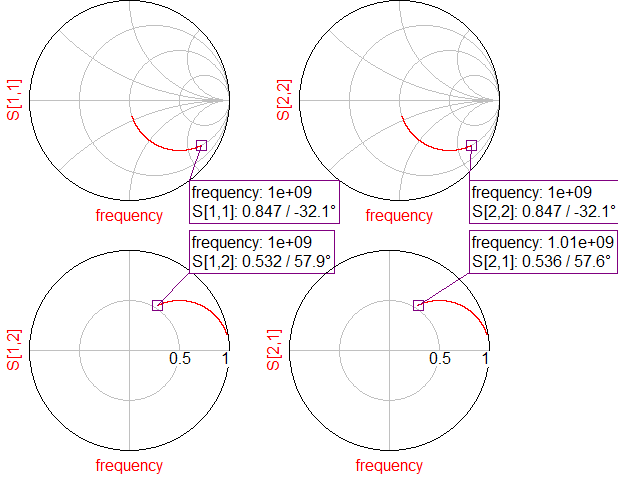
\includegraphics[scale=.5]{Resultados.png}
    \caption{Resultados numéricos da simulação}
    \label{Resul}
\end{figure}

\subsection{Arquivos Touchstone}

Analisando os arquivos Touchstone fornecidos previamente, foi observado que a faixa de freqûencia medida foi de 50MHz à 20GHz.

Fazendo a simulação para este intervalo onde o arquivo \verb L_07C10N_SER.s2p ~é representado na Figura~\ref{Sim2} e o arquivo \verb L-07C10N_SNT.s2p ~na Figura~\ref{Sim3}

\begin{figure}[htbp]
    \centering
    \includegraphics[scale =.5]{simulacao_ser.png}
    \caption{Simulação arquivo SER na frequência válida}
    \label{Sim2}
\end{figure}


\begin{figure}[htbp]
    \centering
    \includegraphics[scale =.5]{simulacao_snl.png}
    \caption{Simulação arquivo SNT na frequência válida}
    \label{Sim3}
\end{figure}


\noindent A seguir interpretando os resultado:

\subsubsection{Comportamentos na baixa frequência:}
\begin{itemize}
    \item A impedância na frequência mais baixa do arquivo \textit{SER} se aproxima ao centro da carta indicando uma comportamente puramente resistivo
    \item No arquivo \textit{SNT}, nas baixas frequência o modelo está num regime de curto circuito.
\end{itemize}

\subsubsection{Comportamento em função da frequência:}
\begin{itemize}
    \item Ao aumentar a frequência do cirtuito \textit{SER} adquire um caráter indutivo até uma frequência de 5 GHz.
    \item Analizando o circuito \textit{SNT}, ele inicialmente possui um comportamento indutivo e após 5 GHz, adquire um comportamento capacitivo, que após a frequência atingir 10 GHZ ele volta ao mesmo caráter indutivo.
\end{itemize}
 
\subsubsection{Ressonâncias:}
\begin{itemize}
    \item Temos que no arquivo \textit{SER} a 5 GHz uma ressonância no indutor.
    \item No arquivo \textit{SNT} temos uma ressonância também em 5 GHz.
\end{itemize}

\subsubsection{Variação das partes imaginárias e reais da impedância:}
\begin{itemize}
    \item No arquivo \textit{SER}, temos que a parte imagniaria implementa um arco seguindo um arco de indutância e capacitânia constante, retornando ao ponto inicial, com a sua parte real acompanhando até um circuito aberto(resistência infinita) e retornando.
    \item No arquivo \textit{SNT}, vemos que o circuito parte de quase um curto e segue um arco de indutância constante até atingir sua ressonância em 5 GHz, enquanto sua parte real vai aumentando também.
\end{itemize}

\subsubsection{Configurações Série ou Paralelo:}
\begin{itemize}
    \item No arquivo \textit{SER}, temos uma conexão de um indutor em série
    \item No arquivo \textit{SNT}, temos uma conexão de um indutor em paralelo, pois a carta parte de um quase curto circuito.
\end{itemize}

\subsection{Modelos propostos}

A seguir é apresentado os modelos propostos para cada arquivo, bem como suas simulações, indicando suas áreas válidas:

\subsubsection{Arquivo SER:}

Na Figura~\ref{modelser} é apresentado um primeiro modelo proposto para o primiro arquivo Touchstone e seu resultado na Figura~\ref{resulSer}, possui uma validade na faixa de 50 MHz até 7Hz.

\begin{figure}[htbp]
    \centering
    \includegraphics[scale =.5]{Modelo1_SER.png}
    \caption{Modelo proposto para o Arquivo SER}
    \label{modelser}
\end{figure}

\begin{figure}[htbp]
    \centering
    \includegraphics[scale=.5]{resultados_modelo1_SER.png}
    \caption{Resultados da simulação sobre o modelo proposto SER}
    \label{resulSer}
\end{figure}

\subsubsection{Arquivo SNT:}

Na Figura~\ref{modelsnl} é apresentado um primeiro modelo proposto para o primiro arquivo Touchstone e seu resultado na Figura~\ref{resulsnl}, possui uma validade na faixa de 50 MHz até 5Hz.

\begin{figure}[htbp]
    \centering
    \includegraphics[scale =.5]{modelo_SNL.png}
    \caption{Modelo proposto para o Arquivo SNT}
    \label{modelsnl}
\end{figure}

\begin{figure}[htbp]
    \centering
    \includegraphics[scale=.5]{resultados_SNL.png}
    \caption{Resultados da simulação sobre o modelo proposto SNT}
    \label{resulsnl}
\end{figure}

\subsection{Fator de Qualidade:}

A seguir plotamos os Fatores de qualiade dos modelos propostos, uilizando a seguinte Equação~\ref{eqn10}. Onde: \[\varDelta F\] é a banda de 3db do máximo e Fr, a frequência de máxima impedância. Os resultados seguem a lógica representados pela Equação~\ref{eqn11}, onde a Eqn.~\ref{eqn11:1} para uma conexão paralela, como no arquivo \textit{SNT} e a Eqn.~\ref{eqn11:2} em série, para o arquivo \textit{SER}. Os gráficos foram gerados utilizando a linguagem \textit{Python} utilizando o compilador \textit{Jupyter} para o processamento dos dados, notebook em anexo, junto como os dados utilizados.  

\begin{equation}
    Q = \frac{F_{r}}{\varDelta F}
    \label{eqn10}
\end{equation}

\begin{subequations}

    \begin{equation}
    Q = R/X 
    \label{eqn11:1}
    \end{equation}

    \begin{equation}
    Q = X/R
    \label{eqn11:2}
    \end{equation}

    \label{eqn11}
\end{subequations}


\subsubsection{Modelo SER:}

A seguir o fator de qualiade do modelo SER representado na Figura~\ref{qualidadeSER}. Podemos observar que o fator Q aumenta com o aumento da frequência que condiz com a expressão~\ref{eqn11:2}, onde com o aumento da frequência tende a aumentar com a frequência e portanto Q possui um aumento proporcional, temos este comportamento pois o nosso modelo não considera que a resistência atuando como uma função da frequência.

\begin{figure}[htbp]
    \centering
    \includegraphics[scale=.5]{Qualidade_SER.png}
    \caption{Fator de Qualiade do modelo SER}
    \label{qualidadeSER}
\end{figure}

\subsubsection{Modelo SNT:}

A seguir o fator de qualiade do modelo SER representado na Figura~\ref{qualidadeSNL}.Podemos indentificar que a frequência de autorressonância de 5.06 GHz que condiz como os experimentos realizados. Podemos observar que até a frequência de ressonância o modelo se comportava como um circuito em paralelo de acordo com a Expressão~\ref{eqn11:1}, no entando no momento que a frequência de análise ultrapassa Fr o modelo passa a se comportar como um circuito em paralelo seguindo a lógica da Expressão~\ref{eqn11:2}.

\begin{figure}[htbp]
    \centering
    \includegraphics[scale=.5]{qualidade_SNL.png}
    \caption{Fator de Qualiade do modelo SNT}
    \label{qualidadeSNL}
\end{figure}


\section{Questões}
\subsection{Questão 1:}

Prove que se pode realizar a conversão entre as matrizes Z e S utilizando a Equação~\ref{eqn6}, onde I é a matriz indentidade.

\begin{equation}
    S = \frac{(Z - Z_{0}I)}{(Z + Z_{0}I)}
    \label{eqn6}
\end{equation}

\textbf{Resolução:}

\noindent Temos as Equações~\ref{eqn1} onde V e I são vetores como a seguir:

\[V = \begin{bmatrix} V_{1}\\ V_{2} \end{bmatrix}~~ \textbf{I} = \begin{bmatrix} I_{1}\\ I_{2} \end{bmatrix}\]

\noindent Temos também que a matriz Z definida a seguir:

\[V = ZI, onde~ Z = \begin{bmatrix} Z_{11} & Z_{12} \\ Z_{21} & Z_{22} \end{bmatrix}\]

\noindent Aplicando a definição V = ZI na parte V + Z0I das Equações~\ref{eqn1} temos que:

\[\begin{bmatrix} V_{1}\\ V_{2} \end{bmatrix}+ Z_{0}\begin{bmatrix} I_{1}\\ I_{2} \end{bmatrix}\rightarrow \begin{bmatrix} Z_{11} & Z_{12} \\ Z_{21} & Z_{22} \end{bmatrix}\begin{bmatrix} I_{1}\\ I_{2} \end{bmatrix} + Z_{0}\begin{bmatrix} I_{1}\\ I_{2} \end{bmatrix}\]

\[\begin{bmatrix} Z_{11}I_{1} + Z_{12}I_{2}\\ Z_{21}I_{1} + Z_{22}I_{2} \end{bmatrix} + \begin{bmatrix} Z_{0}I_{1}\\ Z_{0}I_{2} \end{bmatrix}\rightarrow \begin{bmatrix} Z_{11}I_{1} + Z_{12}I_{2} + Z_{0}I_{1}\\ Z_{21}I_{1} + Z_{22}I_{2} + Z_{0}I_{2} \end{bmatrix}\]

\[\begin{bmatrix} (Z_{11} + Z_{0})I_{1} + Z_{12}I_{2}\\ Z_{21}I_{1} + (Z_{22}+Z_{0})I_{2} \end{bmatrix}\rightarrow \begin{bmatrix} Z_{11} + Z_{0} & Z_{12} \\ Z_{21} & Z_{22}+Z_{0} \end{bmatrix}\begin{bmatrix} I_{1}\\ I_{2} \end{bmatrix}\]

\[\left [ \begin{bmatrix} Z_{11} & Z_{12} \\ Z_{21} & Z_{22} \end{bmatrix} + Z_{0}\begin{bmatrix} 1 & 0 \\ 0 & 1 \end{bmatrix} \right ]\cdot \begin{bmatrix} I_{1}\\ I_{2} \end{bmatrix} = (Z + Z_{0}I)\textbf{I}\]

\noindent Portanto temos que:

\begin{subequations}
    \label{eqn7}
    \begin{equation}
        \label{eqn7:1}
        a = \frac{(Z + Z_{0}I)\textbf{I}}{2\sqrt{Z_{0}}}
    \end{equation}

    \begin{equation}
        \label{eqn7:2}
        b = \frac{(Z - Z_{0}I)\textbf{I}}{2\sqrt{Z_{0}}}
    \end{equation}
\end{subequations}

\noindent Sabemos que S = b/a, logo:

\[S = \frac{(Z - Z_{0}I)}{(Z + Z_{0}I)}\]

\subsection{Questão 2:}
Encontrar a matriz Y (e a matriz S) do quadripolo representado na Figura~\ref{quest2}.

\begin{figure}[htbp]
    \centering
    \includegraphics[scale=.8]{questao2.png}
    \caption{Quadripolo proposto para encontar a Matriz Y e a Matiz S}
    \label{quest2}
\end{figure}

\textbf{Resolução:}

\subsubsection{Cálculo Matriz Y:}

Analisando o nó 1 da Figura~\ref{quest2} e sabendo que Y representa sua admitância, temos que:

\[I_{1} = I_{11} + I_{12}\]

\noindent Onde temos que:
\[I_{11} = (V_{1} - V_{2})Y ~e~ I_{12} = V_{1}Y\]
\noindent Substituindo na equação anterior:

\[I_{1} = (V_{1} - V_{2})Y + V_{1}Y\]

\[I_{1} = 2YV_{1} - YV_{2}\]

\noindent Analogamente para o nó 2, temos que:

\[I_{2} = -YV_{1} + 2YV_{2}\]

\noindent Sabendo que o quadripolo de admitância tem sua forma definida como:

\begin{subequations}
    \label{eqn8}
    \begin{equation}
        \label{eqn8:1}
        I_{1} = Y_{11}V_{1} + Y_{12}V_{2}
    \end{equation}

    \begin{equation}
        \label{eqn8:2}
        I_{2} = Y_{21}V_{1} + Y_{22}V_{2}
    \end{equation}
\end{subequations}

\noindent Comparando os reultados obtidos, temos por comparação a matriz Y a seguir:

\[Y = \begin{bmatrix} 2Y & -Y \\ -Y & 2Y \end{bmatrix}\]

\subsubsection{Cálculo Matriz S:}

Para o cálculo para a a matriz S primeiramente iremos converter a Matriz Z em Y, feito a seguir:

\[\begin{bmatrix} Z_{11} & Z_{12} \\ Z_{21} & Z_{22} \end{bmatrix} = \begin{bmatrix} Y_{11} & Y_{12} \\ Y_{21} & Y_{22} \end{bmatrix}^{-1}\]

\[= \frac{1}{\left | Y \right |}\begin{bmatrix} Y_{22} & -Y_{12} \\ -Y_{21} & Y_{11} \end{bmatrix}, onde~ \left | Y \right | = Y_{11}Y_{22}-Y_{12}Y_{21}\]

\noindent Comparando os resultados e substituindo os valores obtemos:

\[Z = \begin{bmatrix} 2/3~Z & 1/3~Z\\ 1/3~Z & 2/3~Z \end{bmatrix}\]

\noindent Para a o cálculo da matriz S utilizaremos a Eqn.~\ref{eqn6}, feito a seguir:

\[S = (Z - Z_{0}I)(Z + Z_{0}I)^{-1}\]

\noindent Seguindo este raciocício obtemos:

\begin{align*}
    S_{11} = [(Z_{11} - Z_{0})(Z_{22}+Z_{0})-Z_{12}Z_{21}]/\left | Z \right | \\             
    S_{12} = [Z_{12}(Z_{11} + Z_{0}) - Z_{12}(Z_{11} - Z_{0})]/\left | Z \right | \\
    S_{21} = [Z_{21}(Z_{22}+Z_{0}) - Z_{21}(Z_{22}-Z_{0})]/\left | Z \right | \\
    S_{22} = [(Z_{11}+Z_{0})(Z_{22}-Z_{0}) - Z_{12}Z_{21}]/\left | Z \right | \\
    ~ \\
    \left | Z \right | = (Z_{11} + Z_{0})(Z_{22}+Z_{0}) - Z_{12}Z_{21}
\end{align*}

\noindent Utilizando estas equações encontramos:

\begin{align*}
    S_{11} = \frac{\frac{1}{3}Z^{2} - Z_{0}^{2}}{(Z + 4Z_{0})\frac{Z}{3}+Z_{0}^{2}} \\             
    S_{12} = \frac{\frac{2}{3}ZZ_{0}}{(Z + 4Z_{0})\frac{Z}{3}+Z_{0}^{2}}
\end{align*}

Temos por reciprocidade e simetria:

\begin{align*}
    S_{11} = S_{22} ~e~  S_{21} = S_{12}\\
\end{align*}

\subsection{Questão 3:}

Encontrar a matriz Z (e a matriz S) do quadripolo representado na Figura~\ref{quest3}.

\begin{figure}[htbt]
    \centering
    \includegraphics[scale=.8]{questao3.png}
    \caption{Quadripolo proposto para encontar a Matriz Z e a Matiz S}
    \label{quest3}
\end{figure}

\textbf{Resolução:}

\subsubsection{Cálculo Matriz Z:}

Analizando o a malha 1 do circuito na Figura~\ref{quest3}, e sabendo que Z representa sua impedância, temos que:

\[V_{1} - I_{1}Z - Z(I_{1} + I_{2})\]

\[V_{1} = 2ZI_{1} + ZI_{2}\]

\noindent Analogamente para a malha 2, temos:

\[V_{2} = ZI_{1} + 2ZI_{2}\]

\noindent Sabendo que o quadripolo de impedância tem sua forma definida como:

\begin{subequations}
    \label{eqn9}
    \begin{equation}
        \label{eqn9:1}
        V_{1} = Z_{11}I_{1} + Z_{12}I_{2}
    \end{equation}

    \begin{equation}
        \label{eqn9:2}
        V_{2} = Z_{21}I_{1} + Z_{22}I_{2}
    \end{equation}
\end{subequations}


\noindent Comparando os reultados obtidos anteriormente, temos por comparação a matriz Z a seguir:

\[ Z= \begin{bmatrix} 2Z & Z\\ Z & 2Z \end{bmatrix}\]

\subsubsection{Cálculo Matriz S:}

Para o cálculo da Matriz seguimos o mesmo processo de anteriormente e obtemos os seguinte resultados:

\begin{align*}
    S_{11} = S_{22} = \frac{3Z^{2}-Z_{0}^{2}}{(3Z+4Z_{0})Z + Z_{0}^{2}}\\
    S_{12} = S_{21} = \frac{2ZZ_{0}}{(3Z+4Z_{0})Z + Z_{0}^{2}}
\end{align*}

\subsection{Questão 4:}

Sabendo que em circuito em séria segue a lógica como da Equação~\ref{eqn11:2} e como o Fator de Qualidade não varia com a frequência, portanto um valor constante, logo para essa fração citada as trajetórias seriam representados como a Figura~\ref{Qfactor}, para alguns valores de Q definidos.

\begin{figure}[htbp]
    \centering
    \includegraphics[clip=true, trim= 0mm 0mm 0mm 115mm, scale=.2]{Qfactor.png}
    \caption{Trajetórias para o Fator Q}
    \label{Qfactor}
\end{figure}


\subsection{Questão 5:}

Inicialmente, em frequências mais inferiores, o circuito naão teria influências sobre o os componentes, no momento que CA passa a conduzir, os Pads iram começar a conduzir, afetando a corrente original, após o capacitor CB conduzir irá produizir um curto onde o circuito não funcionará mais adequadamente. Portanto sua impedânica com o aumento da freqência irá diminuir.
\noindent A parte imaginária começará no negativo e aumentar, enquanto a parte real vai decair, fazendo que no final a impedância tenda a 0 enquanto a frequência aumenta. Resultado da simulação na Figura~\ref{pads}.

\begin{figure}[htbp]
    \centering
    \includegraphics[scale=.40]{resultado_pads.png}
    \caption{Resultados da análise dos "Pads" em função da frequência}
    \label{pads}
\end{figure}


\subsection{Questão 6:}

Partiria de um circuito aberto, por conta do capacitor, em baixas frequências, fazendo um arco até atingir a frequência de autorressonância, onde, a partir desse ponto, as componentes indutivas terão maior influência sobre o circuito, se deslocando para um circuito aberto novamente, em frequência muito superiores.

\section{Conclusão}

Em conclusão, neste experimento foi analizado as equações de ondas de potência e o uso da simulação de parâmetros S do simulador \textit{QUCS}.
\noindent Foi analizado o uso de arquivos Touchstone para análise e modelamento dos circuitos medidos, analizando suas faixas de frequências válidas, bem como a determinação do Fator de Qualidade.
\noindent Foi analizado de forma mais teórica o uso de diversas matrizes de parâmetros como matriz S, Z, Y bem como suas conversões e aplicabilidade
\noindent Analisamos também os probelemas que os "pads" podem geram num circuito caso não sejamos cuidadosos com as frequências utilizadas nos circuitos 
\noindent Uma pequena análise teórica de como um circuito RLC se comportaria no ábaco de Smith, como também o Fator de Qualidade.

\section{Referências}
\nocite{*}

\bibliographystyle{IEEEtran}
\bibliography{Lab_02}

\end{document}